% !TEX TS-program = pdflatex
% !TEX root = main.tex
\documentclass[12pt,a4paper, oneside]{article} %international style

% adjusting margins for standard university paper
\usepackage[left=2cm, right=4cm, top=2cm, bottom=2cm]{geometry}

%other packages (put here whatever else is needed)
\usepackage[nswissgerman]{babel}
\usepackage[utf8]{inputenc}
\usepackage{graphicx} %images
\usepackage[bookmarks=true,colorlinks=true]{hyperref} %hyperlinks
\usepackage{calc} %position calculation
\usepackage{amsmath} %math symbols
\usepackage{lucide-icons} %lucide icons
\usepackage{longtable}
\usepackage{multirow}
\usepackage[T1]{fontenc}
\usepackage{helvet}
\renewcommand{\familydefault}{\sfdefault}

\usepackage{fancyhdr} % Load the package

\fancypagestyle{style}{
\fancyhf{} % Clear existing headers and footers
\fontsize{9pt}\selectfont % Set font size for header and footer
\fancyhead[L]{\@title}
\fancyhead[R]{Universität Fribourg \\ FS 2026}
\fancyfoot[L]{\date{\today}}
\fancyfoot[C]{\fontsize{11pt}\selectfont \thepage} % Centered page number in footer
\fancyfoot[R]{Leo Spack}
\renewcommand{\headrulewidth}{0.4pt} % Line below header
\renewcommand{\footrulewidth}{0.4pt} % Line above footer
}

%---
%AUTHOR AND TITLE
\author{Leo Spack}
\title{Die römische Republik bis zur sogenannten Gracchenkrise}
\date{\today}
%---
%ADDITIONAL INFO FOR PDF
\pdfinfo{
/Title (Die römische Republik bis zur sogenannten Gracchenkrise)
/Author (Leo Spack)
/Subject (Zusammenfassung der römischen Republik bis zur sogenannten Gracchenkrise)
/Creator (LaTeX)
/Producer (PDFLaTeX)
/CreationDate (\today)
/Keywords (Römische Republik, Gracchenkrise, Zusammenfassung)
}

\begin{document}
%---TITLE PAGE
\begin{titlepage}
\begin{center}

\hrule{0.5pt.}\\[0.3cm]
\textsc{\Large Leo Spack} \\[0.3cm]
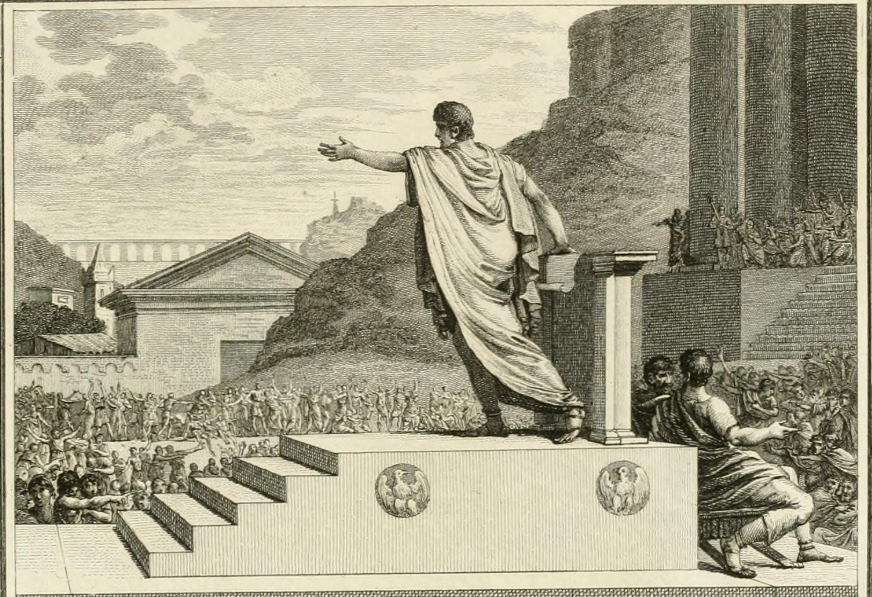
\includegraphics[width=8.5cm]{img/tiberius-and-gaius-gracchus.jpg} \\[0.3cm]
%Title
{ \Huge \bfseries Die römische Republik bis zur sogenannten Gracchenkrise \\[0.1cm] \Large Zusammenfassung \HRULE \\[0.3cm]}

\end{center}
\end{titlepage}

\tableofcontents
\newpage
\pagestyle{style} % Apply the custom page style to the rest of the document
\setcounter{page}{1}

\chapter{18.02. Einführung in die Epochen und Vorstellung der Quellen}
placeholder

\end{document}